\hypertarget{ikkuna}{%
\chapter{Ikkuna}\label{ikkuna}}

Ikkuna is the Python library developed for this thesis. It targets
Python 3.6 and was designed with the following goals in mind:

\begin{enumerate}
    \item
        Ease of use through minimal configuration overhead
    \item
        Flexible and all-encompassing API enabling creating arbitrary metrics
        which act on training artifacts
    \item
        Metrics shall be agnostic of model code.
    \item
        Plugin architecture so metrics written once can be used for any kind
        of model
    \item
        Framework agnosticism. Ideally, the library would support every deep
        learning framework through an extensible abstraction layer.
\end{enumerate}

What it provides over the aforementioned tools (\cref{sec:existing-apps}) is that it enables
working at a higher level of abstraction, liberating the developer from
having to repeat herself, exchanging visualisations and metrics and
reduce the friction between development and debugging.

This chapters gives a
high-level overview of the library components and elaborates on the design
decisions made during the creation. Throughout the chapters, UML class and
package diagrams will serve as a mental map for the reader. For brevity, not all
parts of the library are diagrammed down to the same level of detail.

\hypertarget{design-principles}{%
\section{Design Principles}\label{design-principles}}

Of the aforementioned goals, all except one have been accomplished. The
objective of making the library agnostic to the deep learning framework
being used (TensorFlow, PyTorch, PyCaffe, Chainer, etc.) has been
neglected for practical reasons. Enabling this kind of support is beyond
the scope of this thesis and only requires the implementation of a
software layer which offers framework-agnostic access to network
modules, activations, gradients and all the other necessary information.
While this is certainly possible and useful, the PyTorch framework has
been chosen for this work to create a proof of the concept. The choice is
motivated in \cref{sec:dl-frameworks}.

The overarching architecture of this software must lend itself to this
agnosticity goal, however. As such, a very loose coupling between model code,
metric computation and visualisations is desired. Not only will this aid in
extending the library to different deep learning frameworks, but it is also a
prerequisite for allowing for modular, self-contained visualisations or metrics
which can be installed and used separately and independently of specific model
code. The Publisher-Subscriber design pattern has been chosen for these reasons
(\cref{sec:pubsub}).

\hypertarget{sec:dl-frameworks}{%
\section{Deep Learning frameworks}\label{sec:dl-frameworks}}

As neural networks are essentially sequences of matrix operations and
elementwise function application followed by reduction operations, deep learning
frameworks are not much different from previously available matrix libraries
such as Eigen or NumPy. The value they provide lies in the fact that they
embrace the concept of automatic differentiation and GPU acceleration. Unless
specifically noted, all operations provided by these libraries are accompanied
by their respective derivatives and a mechanism is provided to apply the chain
rule to arbitrary sequences of operations in order to compute the derivative of
their output with respect to the inputs.

All frameworks have in common that they build a graph representation of the
model, whether implicitly or explicitly, and use it to parallelise propagations
and factor dependencies into paths for computing derivatives in parallel. Nodes
in the graph are operations while edges are data flowing between operations.
This allows naturally parallelising independent computations. To compute
gradients, the graph can be traversed backwards from the output node by applying
the reverse-mode autodifferentiation algorithm (a generalisation of the plain
backpropagation used in the multilayer perceptron).  Define-and-run frameworks
like TensorFlow create the graph explicitly; the user uses the API to do exactly
this. The graph -- once compiled -- is fixed for the entire training process.
PyTorch on the other hand implicitly records all operations as they execute and
also overloads arithmetic operators for this purpose. The graph is recreated for each
propagation through the network and the user never directly interacts with it.
This precludes some optimizations, but makes dynamically changing networks
easily achievable.

The currently available deep learning libraries can be located on a spectrum
between define-by-run and define-and-run.  The first extreme would be
frameworks such as PyTorch \citep{paszke2017automatic} or Chainer
\citep{tokui2015chainer} , where there exist no two distinct execution phases --
just as in an ordinary matrix library like NumPy, each statement immediately
returns or operates on an actual value. By contrast, frameworks like
TensorFlow\footnote{Since version 1.4, TensorFlow gravitates toward
    define-by-run through the introduction of \emph{eager execution}, which
becomes the default mode in version 2.0. Graph-based execution is still
available, but not the default any longer.} require specifying the model graph
in a domain-specific language (TensorFlow has Python, Java and C++ APIs, Caffe
uses Prototxt files), compile it to a different representation and the model
is run and trained in a second phase. While this enables graph-based
optimizations, the main downsides are that

\begin{itemize}
    \item
        control flow cannot use the host language features, but must be done
        with the API used for defining models. Instead of
        \begin{lstlisting}[language=Python, label=lst:whilepy-pt, gobble=8]
        counter = torch.tensor(0)
        # repeated matrix multiplication
        while counter < tensor:
            counter += 1
            h = torch.matmul(W, h) + b
        \end{lstlisting}

        one must use a construction like this
        \begin{lstlisting}[language=Python, label=lst:whilepy-tf, gobble=8]
        counter = tf.constant(0)
        while_condition = lambda counter: tf.less(counter, tensor)
        # loop body
        def body(counter):
            h = tf.add(tf.matmul(W, h), b)
            # increment counter
            return [tf.add(counter, 1)]

        # do the actual loop
        r = tf.while_loop(while_condition, body, [counter])
        \end{lstlisting}
    \item
        As a corollary, the barrier of entry is higher, since a beginner cannot rely on the
        language feature she knows but must learn how to express many concepts
        without the host language.
    \item
        halting execution at arbitrary points in the training is not possible,
        since the actual training is not happening in the host language, but
        is more often handed off to lower-level implementations in its
        entirety.
\end{itemize}
This makes conditional processing and debugging much less ergonomic.

For this work, the PyTorch framework has been chosen, due to the fact
that it is growing quickly in popularity (see \cref{fig:popularity}) and
relatively new, so the ecosystem is not fully developed and some
utilities available for e.g.~TensorFlow are not available for PyTorch.
Because of this, an introspection framework for training monitoring is
judged to present the best value proposition for PyTorch users.

\begin{figure}
    \hypertarget{fig:popularity}{%
        \centering
        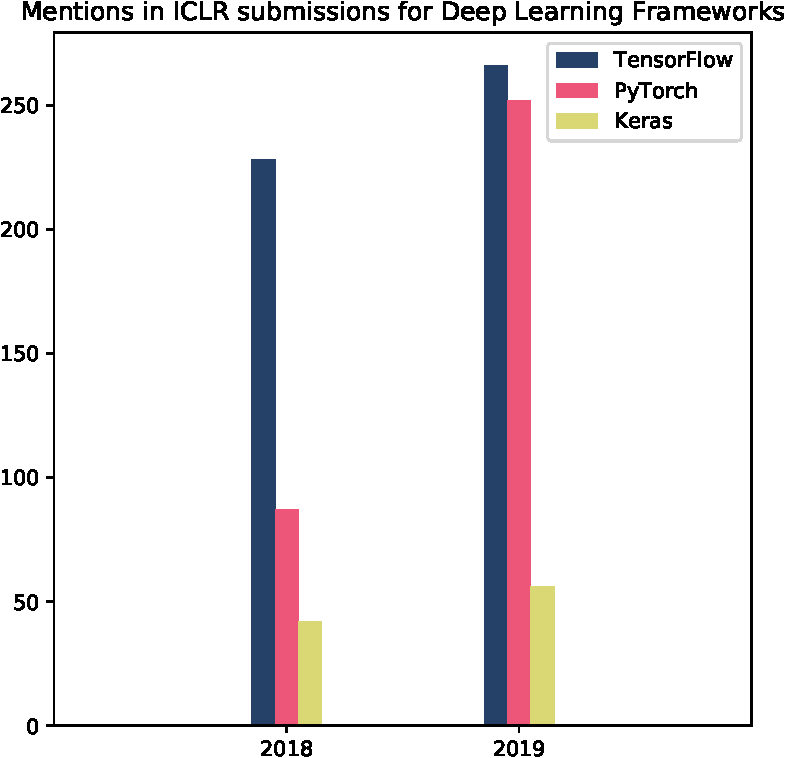
\includegraphics[max width=\textwidth]{gfx/diagrams/framework_popularity/popularity.pdf}
        \caption[Changes in popularity of different deep learning libraries in
        research]{Changes in popularity of different deep learning libraries in
            research. Data was collected by keyword search over ICLR submissions
            (\href{http://search.iclr2019.smerity.com/search/}{http://search.iclr2019.smerity.com/search};
        analogously for 2018)}\label{fig:popularity}
    }
\end{figure}

\hypertarget{sec:pubsub}{%
\section{Publisher-Subscriber}\label{sec:pubsub}}

The Publisher-Subscriber pattern (for a detailed overview see
\cite{eugster2003}) is a pattern for distributed computation in which publishers
publish messages either directly to any subscribers which have registered
interest in them, or to a central authority orchestrating the exchange. Messages
are generally associated with one or more topics and subscribers register
interest in receiving messages on one or more topics.

The components are very loosely coupled; the subscribers need not even
be aware of the publishers at all, and the publishers' only interaction
with their subscribers is relaying messages through a uniform interface
or through an optional server. A graphical schema of one possible
incarnation of this pattern is shown in \cref{fig:pubsub}.

\begin{figure}
    \hypertarget{fig:pubsub}{%
        \centering
        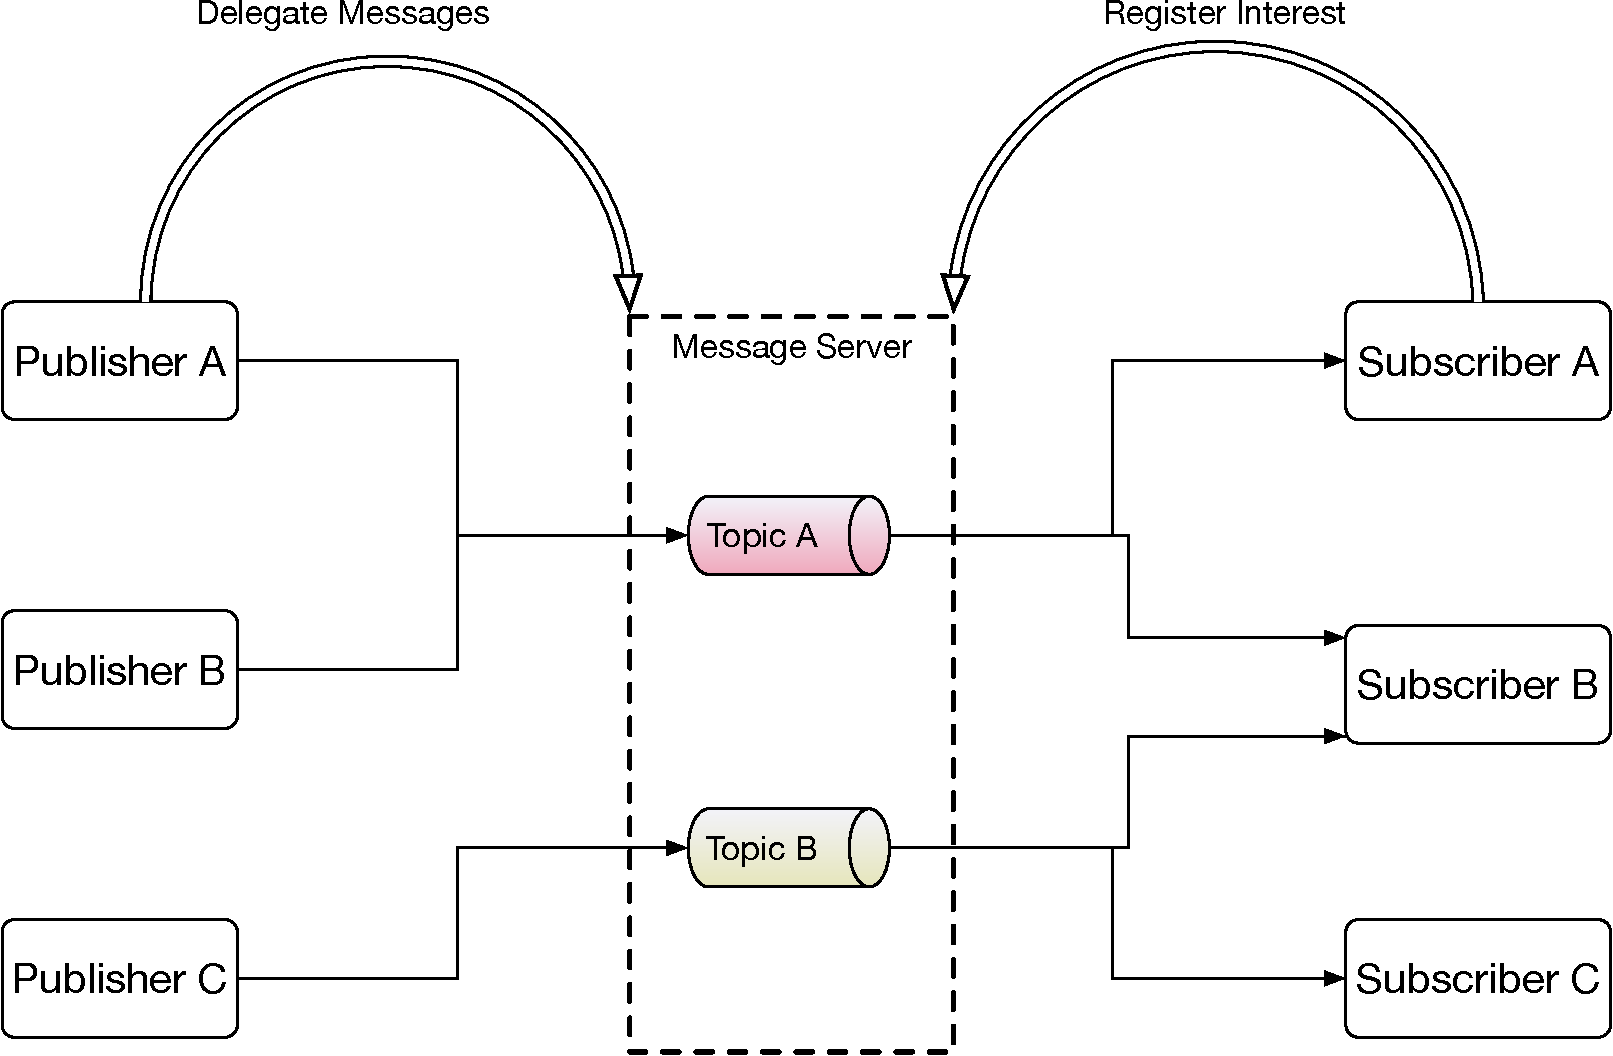
\includegraphics[max width=\textwidth]{gfx/diagrams/architecture_diagrams/pubsub.pdf}
        \caption{One possible implementation of the Publisher-Subscriber pattern.}\label{fig:pubsub}
    }
\end{figure}

This project is not distributed, but can benefit from the loose coupling
in another way: Subscribers can be defined in terms of the kind of
messages they need to compute their metric, without knowing anything
about where the messages are coming from. Concretely, as long as the
appropriate data is emitted from the training process, subscribers can
work without modifications with any possible model.

Since real-world neural networks are trained on the GPU, and communication
between host and GPU memory is already expensive, making this library truly
distributed across processes is not an objective. However, the design will
simplify asynchronous computation of metrics in the future. The Python language
does not support true multithreading\footnote{The \texttt{multiprocessing}
    module allows for truly asynchronous computation and communication, but the
    inter-process-communication is more expensive than memory shared between
threads.}, but since the expensive part of the work is running on the GPU while
the host code is waiting (or prefetching data), metric computation could happen
asynchronously on the GPU as well while the expensive forward or backward passes
through the network are running. This is not currently implemented but can be
added later, in case more computationally demanding metrics are to be explored.

In the context of neural network training, there is only one source of
information -- the model -- and hence only one publisher. Nevertheless, a message server is
introduced to segregate responsibilities. The singular publisher extracts data from the
training model, passes it on to the server which also accepts subscriber
registrations and relays messages appropriately.

\hypertarget{overview-of-the-library}{%
\section{Overview of the library}\label{overview-of-the-library}}

The software is structured into several packages. The root package is
\texttt{ikkuna} which encapsulates all core
functionality. All other packages and modules contain utilities
implemented for this work specifically, but will generally not be
relevant to other users. A survey of these tools will be given in
\cref{sec:other-tools}. This section surveys the structure of the codebase and
elaborates on implementation strategies, but does not constitute a full
documentation. For a detailed API reference, the reader is referred to the HTML
documentation\footnote{At the time of writing located at \url{https://peltarion.github.io/ai_ikkuna/}}.

The root package diagram is shown in \cref{fig:pack-diag-ikkuna}

\begin{figure}
    \hypertarget{fig:pack-diag-ikkuna}{%
        \centering
        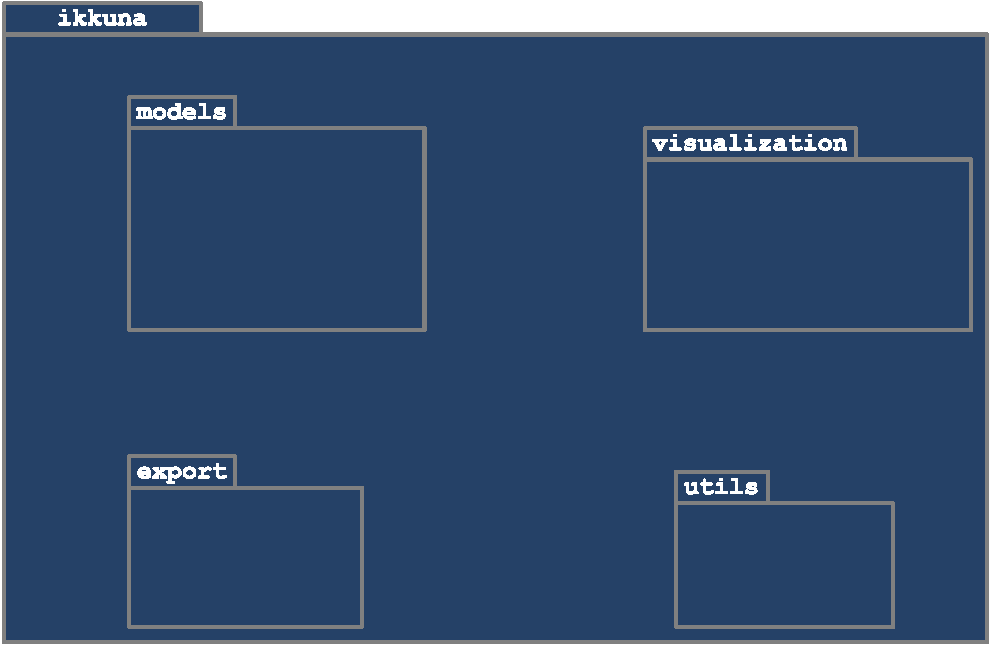
\includegraphics[max width=.7\textwidth]{gfx/diagrams/class_diagrams/ikkuna_package_diagram.pdf}
        \caption{\texttt{ikkuna} package diagram}\label{fig:pack-diag-ikkuna}
    }
\end{figure}

The most important bits of the software live in the
\texttt{export} subpackage (\cref{sec:pack-export}). It
implements the Publisher-Subscriber pattern. Extracting data from the
training process, defining subscriber functionality and messages used
for communication is done here.

The \texttt{models} (see \cref{sec:pack-models}) subpackage contains a few
exemplary neural network definitions which are wired up with the library and can
thus be used to showcase the library's functionality. The \texttt{utils} (see
\cref{sec:pack-utils}) subpackage contains miscellaneous utility classes and
functions used throughout the core library. Lastly, the \texttt{visulization}
subpackage (\cref{sec:pack-visualization}) contains the plotting functionality
to actually show the metrics computed during the training process.

\hypertarget{sec:pack-export}{%
\subsection{The \texttt{export} subpackage}\label{sec:pack-export}}

The \texttt{export} subpackage contains the core part
of the library, i.e.~it provides the classes that handle discovering the
structure of the neural network model, attaching the appropriate
callbacks and intercepting method calls on the model so the library is
informed about everything entering and exiting the model and its
individual layers. It also contains the definition for the subscriber
API, i.e.~the messages that subscribers can receive, synchronisation
facilities when multiple topics are needed by a subscriber, as well as
the subscriber class interface. The package diagram is displayed in
\cref{fig:pack-diag-export}.

The package comprises three subpackages or modules listed in
\cref{tbl:ikkuna.export}

\begin{table}
    \caption{\texttt{ikkuna.export} functionalities}
    \label{tbl:ikkuna.export}
    \begin{tabularx}{\textwidth}{lX}
        \toprule
        Name                & Function\tabularnewline
        \midrule
        \texttt{export}     & Define the publisher discovering an arbitrary model and relaying messages to the message server\tabularnewline
        \texttt{messages}   & Define message interface; i.e.~what topics exist and which information a message must contain\tabularnewline
        \texttt{subscriber} & Define the base class for subscribers and classes for message synchronisation and filtering\tabularnewline
        \bottomrule
    \end{tabularx}
\end{table}

\subsubsection*{The \texttt{ikkuna.export} subpackage}

\begin{figure}
    \hypertarget{fig:pack-diag-export}{%
        \centering
        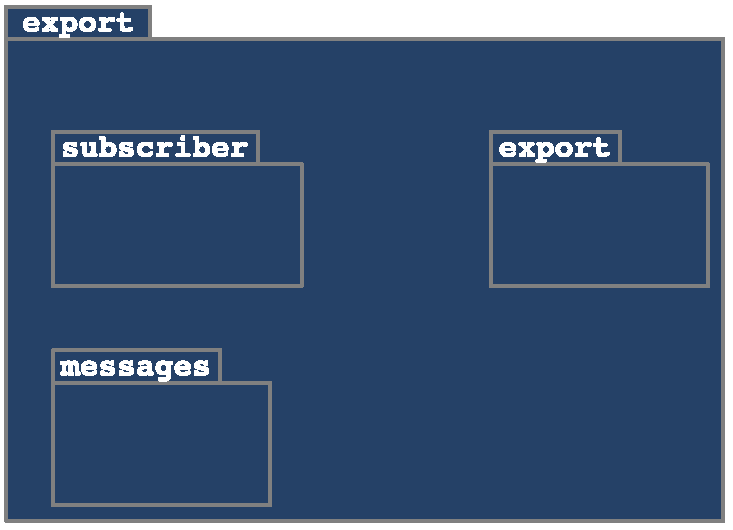
\includegraphics[max width=.7\textwidth]{gfx/diagrams/class_diagrams/export_package_diagram.pdf}
        \caption{\texttt{ikkuna.export} package diagram}\label{fig:pack-diag-export}
    }
\end{figure}

In in slight deviation from the Publisher-Subscriber framework as displayed in
\cref{fig:pubsub}, the \texttt{export.Exporter} class
(\cref{fig:class-diag-exporter}) is the sole publisher of data. There is only one
source of data during training, so it is unnecessary to accommodate multiple
publishers. The \texttt{Exporter} is informed of the model with its methods
\lstinline{set_model()} and \lstinline{set_loss()}, the latter of which is only
necessary if metrics which rely on training labels should be displayed.  It can
accept a filter list of classes which are to be included when discovering the
modules in the model. For instance, it could be desirable to only observe layers
which have weights and biases associated with them, not e.g.~normalisation or
reshaping layers. The \texttt{Exporter} then traverses the model (which is
really just a tree structure of modules) and adds to each a callback invoked
when input enters the layer -- in order to retrieve activations -- and when
gradients are computed for the layer outputs. PyTorch provides the
\lstinline+add_forward_hook()+ and \lstinline+add_backward_hook()+ functions on
modules (layers) and \lstinline+add_hook()+ function on Tensors to register
callbacks. All added modules are also given a name -- either set by the user
during creation of the model or generated automatically. The name is necessary
for display purposes.

The callbacks also use cached weights -- if present -- in order to publish updates to the weights.

Furthermore, the \lstinline+Exporter+ employs monkey patches to the model; it
replaces a few of the model's methods with closure wrappers -- functions defined
locally which have access to the \lstinline+Exporter+ instance -- so it can

\begin{itemize}
    \item
        be notified when the model is set to training or testing mode (this
        switch disables or enables layers which only make sense during one of
        the phases\footnote{There are two built-in layers this applies to. One
            is the batch normalisation layer. It normalises the output of the
            previous layer with the mean and variance over the entire batch of
            data -- optionally with running means and variances over the
            previous training steps. The variance is not defined for
            single data point enters the layer, as could be the case during
            inference/testing time. The second case is the dropout layer, which
            randomly zeroes out a percentage of the previous layer's
            activations. This is used during training to prevent subsequent
            units from becoming correlated with a fixed set of units in the
            previous layer, instead of picking up patterns invariant of where in
            the input they occur. During inference time, this is turned off to
            make full use of the trained
        layers.})
    \item
        increase its own step counter automatically when a new batch is seen.
        This can be deduced from the fact that \lstinline+forward()+ is called
        on the model.
    \item
        add a parameter to the model's \lstinline{forward()} method -- called by
        the runtime when data is propagated through the model -- which can be
        used be subscribers to temporarily turn off training mode and have it
        revert automatically. This is useful for subscribers which need to
        evaluate the model and are thus given limited access through the
        \lstinline+forward()+ method, but do not want the \lstinline+Exporter+
        to generate new messages for this occasion (this could even lead to
        infinite loops).
    \item
        intercept inputs and labels passed to the loss function during training and
        publish them as messages so the user need not concern himself with
        this task. This is useful for e.g. computing the accuracy on the current
        batch with the subscriber framework.
    \item
        intercept the final output of the network. This could be realised
        alternatively by identifying the last module in the network, but is
        easier to do by patching the loss function set with
        \lstinline+set_loss()+.
\end{itemize}

At every time step (training batch), the \texttt{Exporter} publishes the
following information on to the message bus (see \cref{fig:messages_class_diag}):

\begin{itemize}
    \item
        gradients for each module
    \item
        gradients for each parameter (loss derivative w.r.t the weights and biases)
    \item
        activations for each module
    \item
        current values of weights and biases for each module that has these properties
        (e.g.~convolutional or fully-connected layers)
    \item
        updates to the weights and biases applied at the end of the current
        step
    \item
        Training labels used for the parameter updates. This requires that the
        \texttt{Exporter} be informed of the loss function object with
        \lstinline{set_loss()}.
    \item
        The batch of input data passed to the network at the current training step
    \item
        The final output of the network for the current batch of training data.
        This is simply the tensor of activations from the last layer and is thus
        technically duplicated since activations are published anyway. The
        reason is that some subscribers may only be interested in the network
        predictions and it is unnecessary to determine automatically the last
        layer in the network as the loss function has automatic access to
        the activations and must be patched anyway for the training labels
\end{itemize}

Further messages are published only at certain points in the training process

\begin{itemize}
    \item
        When a batch starts or ends, a message with the current batch index is published
    \item
        When an epoch starts or ends, a message with the current epoch index is
        published. This requires the \texttt{Exporter} be notified with
        \lstinline{epoch_finished()} by the user, since it is impossible to
        determine when an epoch is over from inside the model.
\end{itemize}

\subsubsection*{The \texttt{ikkuna.export.messages} submodule}

This submodule contains definitions of all permissible messages kinds, message
classes and a collection class for message objects. An overview of the classes
defined in this module is shown in \cref{fig:messages_class_diag}.

\begin{figure}
    \centering
    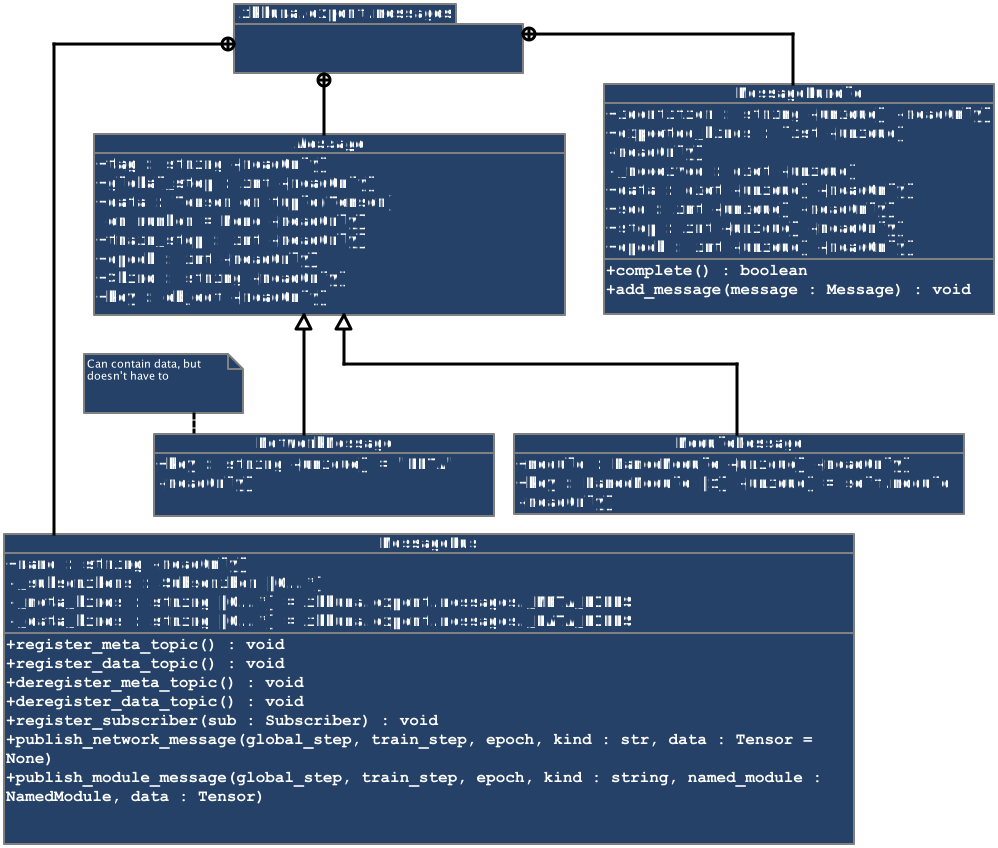
\includegraphics[width=\textwidth]{{gfx/diagrams/class_diagrams/ikkuna.export.messages}.pdf}
    \caption{Classes in the \texttt{ikkuna.export.messages} submodule}
    \label{fig:messages_class_diag}
\end{figure}

Messages are of one of two types: They are either directly tied to a layer in
the network and are thus published for each layer, or they contain information
for the current training step applying to the entire network. In that case, they
appear only once per training step, not once per layer. The meta-messages can
carry tensor data (e.g.~input data or labels), but need not to
(e.g.~notifications about a starting or ending epoch). All message kinds are
summarised in \cref{tbl:messages}.

Messages can be assembled into bundles if a subscribers wants to subscribe
several topics at once. The \texttt{MessageBundle} class performs all necessary
error checking to ensure consistency of the contained messages (only messages of
from the same time step are allowed).

The message server from \cref{fig:pubsub} is implemented by the
\texttt{MessageBus} class which receives publishers' messages, accepts
subscribers registrations, and maintains the lists of known topics. Each
subscriber may in turn announce one or more new topics which can then be
subscribed to by others. This is useful since it allows chaining of subscribers
in order to realise arbitrary post-processing of computed metrics.

\begin{table}
    \centering
    \caption{Subscribable message kinds}
    \label{tbl:messages}
    \begin{tabularx}{\textwidth}{llX}
        \toprule
        \rowcolor{verylightblue}\multicolumn{3}{c}{Meta topics} \tabularnewline
        \midrule
        Identifier                     & Frequency                & Description \tabularnewline
        \midrule
        {\lstinline!batch_started!}    & Once every batch         & \tabularnewline
        {\lstinline!batch_finished!}   & \ditto                   & \tabularnewline
        {\lstinline!epoch_started!}    & Once every epoch         & \tabularnewline
        {\lstinline!epoch_finished!}   & \ditto                   & \tabularnewline
        {\lstinline!input_data!}       & Once every batch         & \tabularnewline
        {\lstinline!input_labels!}     & \ditto                   & \tabularnewline
        {\lstinline!network_output!}   & \ditto                   & Activations of the last layer \tabularnewline
        {\lstinline!loss!}             & \ditto                   & Loss over the current batch \tabularnewline
        \bottomrule
        \rowcolor{verylightblue}\multicolumn{3}{c}{Data topics} \tabularnewline
        \midrule
        Identifier                     & Frequency                & Description \tabularnewline
        \midrule
        {\lstinline!weights!}          & Once per layer per batch & Gradients of loss function w.r.t. layer weight matrix \tabularnewline
        {\lstinline!weight_gradients!} & \ditto                   & \tabularnewline
        {\lstinline!weight_updates!}   & \ditto                   & \tabularnewline
        {\lstinline!biases!}           & \ditto                   & Gradients of
        loss function w.r.t. layer bias vector \tabularnewline
        {\lstinline!bias_gradients!}   & \ditto                   & \tabularnewline
        {\lstinline!bias_updates!}     & \ditto                   & \tabularnewline
        {\lstinline!activations!}      & \ditto                   & \tabularnewline
        {\lstinline!layer_gradients!}  & \ditto                   & Gradients of loss function w.r.t. layer output \tabularnewline
        \bottomrule
    \end{tabularx}
\end{table}

\begin{figure}
    \hypertarget{fig:class-diag-exporter}{%
        \centering
        \includegraphics[max width=.8\textwidth]{gfx/diagrams/class_diagrams/{ikkuna.export.Exporter}.pdf}
        \caption{\texttt{ikkuna.export.Exporter} class diagram}\label{fig:class-diag-exporter}
    }
\end{figure}

\subsubsection*{The \texttt{ikkuna.export.subscriber} subpackage}

The third subpackage contained in the \texttt{ikkuna.export} package defines the
subscriber part of the Publisher-Subscriber pattern. The diagram of the defined
classes is shown in \cref{fig:class-diag-subscriber}. The \texttt{Subscriber}
base class is rudimentary and mandates only the implementation of the metric
computation by subclasses. In the simplest case, a subscriber is interested in
only one topic and therefore is coupled to a simple \texttt{Subscription}
object, which handles bookkeeping tasks such as subsampling the message stream,
routing only relevant messages to the subscriber and counting the received messages.

More generally however, a subscriber may want to receive several pieces of
information for each layer in each time step (i.e.~for computing the ratio
between weight updates and weights). Since the order of messages is not
guaranteed, the desired messages are unlikely to occur one after the other;
instead the topics must be synchronised. A \texttt{SynchronizedSubscription}
buffers messages of the relevant topics until all requested kinds have been
received for the current training step, before releasing them to the subscriber.

A subscriber can thus receive a single message or a bundle of messages for each
subscription. It can also have multiple subscriptions, but each topic can only
be associated with one subscription.

The library comes with a few subscribers already installed (they are themselves
plugins, see \cref{plugin-infrastructure}). Details are given in
\cref{tbl:subscribers}

\begin{figure}
    \centering
    \includegraphics[width=\linewidth]{gfx/diagrams/class_diagrams/{ikkuna.export.subscriber}.pdf}
    \caption{Classes defined in \texttt{ikkuna.export.subscriber}}
    \label{fig:class-diag-subscriber}
\end{figure}

\begin{table}
    \centering
    \caption{Pre-packaged subscriber subclasses}
    \label{tbl:subscribers}
    \begin{tabularx}{\textwidth}{lX}
        \toprule
        Name                             & Functionality                                                                                                                                                         \tabularnewline
        \midrule
        \texttt{MeanSubscriber}          & Computes the mean $\mu = \frac{1}{n}\sum_{i=1}^n w_i$ of a tensor                                                                                                     \tabularnewline
        \texttt{VarianceSubscriber}      & Computes the variance $\sum_{i=1}^n (w_i - \mu)^2$ for a tensor                                                                                                       \tabularnewline
        \texttt{HessianEigenSubscriber}  & The top-$k$ eigenpairs of the Hessian matrix \tabularnewline
        \texttt{NormSubscriber}          & Computes the $p$-Norm $\sqrt[p]{\sum_{i=1}^n w_i^p}$                                                                                                                  \tabularnewline
        \texttt{RatioSubscriber}         & Computes the ratio of norms $\frac{||T_1||_2}{||T_2||_2}$ of two tensors \tabularnewline
        \texttt{HistogramSubscriber}     & Computes the histogram of a given tensor. This is computationally heavy.                                                                                              \tabularnewline
        \texttt{SpectralNormSubscriber}  & Computes the spectral norm (largest singular value) $\max_{\mathbf{h}:\mathbf{h}\neq 0} \frac{\left||A\mathbf{h}\right||_2}{\left||\mathbf{h}\right||_2}$ of a tensor reshaped to $2$-d \tabularnewline
        \texttt{TestAccuracySubscriber}  & Computes the ratio of correctly classified examples to total examples over the test set                                                                               \tabularnewline
        \texttt{TrainAccuracySubscriber} & Computes the ratio of correctly classified examples to total examples over current batch of training data                                                             \tabularnewline
        \bottomrule
    \end{tabularx}
\end{table}

\hypertarget{sec:pack-models}{%
\subsection{The \texttt{models} subpackage}\label{sec:pack-models}}

\begin{figure}
    \hypertarget{fig:pack-diag-models}{%
        \centering
        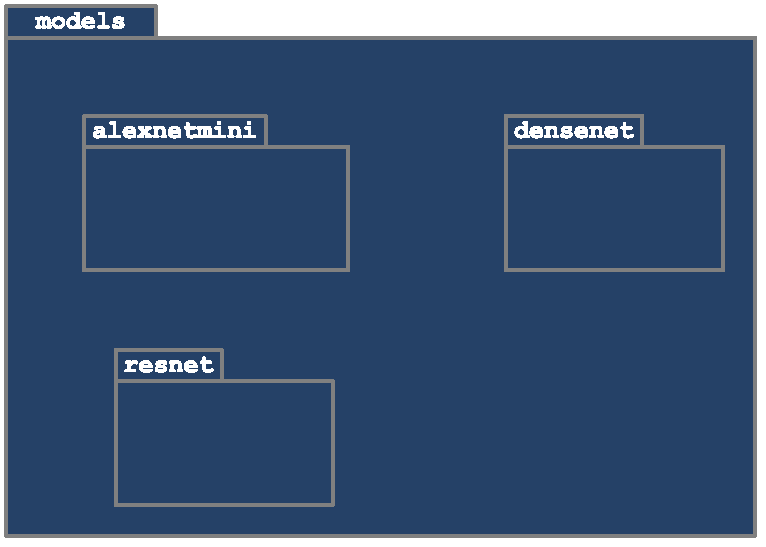
\includegraphics[max width=.7\textwidth]{gfx/diagrams/class_diagrams/models_package_diagram.pdf}
        \caption{\texttt{ikkuna.models} package diagram}\label{fig:pack-diag-models}
    }
\end{figure}

This package shown in \cref{fig:pack-diag-models} contains model
definitions for demonstration purposes and for experimentation. Four
architectures are currently implemented:

\begin{enumerate}
    \item
        A minified version of AlexNet, since the original architecture
        requires larger images \citep{krizhevsky2012imagenet}. The
        code is adapted from Suki
        Lau\footnote{\url{https://github.com/sukilau/Ziff-deep-learning/blob/master/3-CIFAR10-lrate/CIFAR10-lrate.ipynb}}.
    \item
        DenseNet \citep{huang2017densely}. The implementation is basically the
        one from \citep{pleiss2017memory}\footnote{At the time of writing, the
            implementation is available here:
            \url{https://github.com/gpleiss/efficient_densenet_pytorch/blob/master/models/densenet.py}.
            The licensing is unclear as the author references the original
            BSD-licensed implementation at
            \url{https://github.com/pytorch/vision/blob/master/torchvision/models/densenet.py}
            which was licensed by PyTorch core contributor Soumith Chintala.
            However, the code does not reproduce the BSD license text and can
            thus only be inspired by the original but cannot contain any of the
        code verbatim. It would require careful examination in order to
    determine whether this is the case.} with minor modifications
    \item
        ResNet \citep{he2016deep}. This implementation comes from
        GitHub user liukang\footnote{The implementation is MIT-licensed.
        \url{https://github.com/kuangliu/pytorch-cifar/blob/master/models/resnet.py}}
        and can handle CIFAR10-sized images of 32 pixels per side, as opposed
        to most implementaions that are geared towards ImageNet examples which
        are much larger.
    \item
        VGG18, a variant of the deep convolutional network introduced in
        \citep{simonyan2014very}. The code is adapted from the PyTorch model
        zoo's implementation (BSD license).
\end{enumerate}
All models are modified such that their training can be supervised by
the library.

\hypertarget{sec:pack-utils}{%
\subsection{The \texttt{utils} subpackage}\label{sec:pack-utils}}

As shown in \cref{fig:pack-diag-utils}, this package defines classes for
traversing a model into a hierarchical tree of layers (called \emph{modules} in
PyTorch lingo) with some added metadata, and a set of miscellaneous functions for

\begin{enumerate}
    \item
        Seeding random number generators to make experiments reproducible (see
        \cref{ch:appendixB})
    \item
        Creating instances of weight optimizers by name
    \item
        Loading datasets and inferring all metadata about it
    \item
        Creating models by name
    \item
        Initialize the weights of any model
\end{enumerate}

\begin{figure}
    \hypertarget{fig:pack-diag-utils}{%
        \centering
        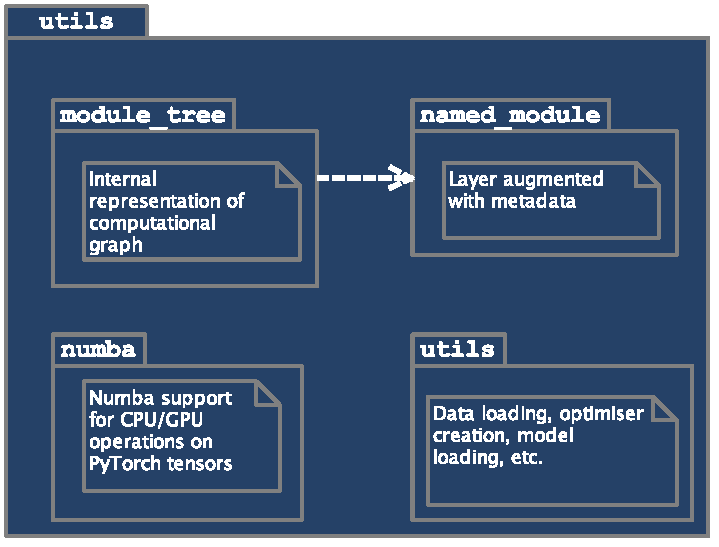
\includegraphics[max width=.7\textwidth]{gfx/diagrams/class_diagrams/utils_package_diagram.pdf}
        \caption{\texttt{ikkuna.utils} package diagram}\label{fig:pack-diag-utils}
    }
\end{figure}

Additionally, it contains the \texttt{numba} module
which is intended to allow interoperability with the Numba
library\footnote{\url{https://numba.pydata.org/}. Numba is a library for
    transforming high-level Python code into performant compiled code and
    for allowing to use the CUDA library from Python with Python arrays.
    This enables performance improvements for numeric calculations, but
    there is only a limited set of higher-level functions implemented on
GPU arrays.}. While currently not used due to the incomplete nature of
the Numba GPU array interface, it could enable leveraging Numba in the
future without transferring data to the CPU. The core function was later
obsoleted by an addition to the PyTorch library\footnote{The main contribution
of the submodule was to make PyTorch tensors accessible to Numba by
monkey-patching the \lstinline{__cuda_array_interface__} property. This has since
been added via pull request \#11984 to the PyTorch repository.}.

\hypertarget{sec:pack-visualization}{%
\subsection{The \texttt{visualization} subpackage}\label{sec:pack-visualization}}

This package contains only a single module: \texttt{backend}. It defines the
classes shown in \cref{fig:class-diag-backend}. The module serves as an
abstraction over plotting libraries (or more generally, information sinks) so
that metrics need not concern themselves with how the data is actually presented
to the user.  A given metric will compute its value and dispatch it to its
backend, which can currently accept scalar and histogram data. The metric class
itself need not care about how it is going to be displayed. While not currently
implemented, monitoring or database backends (e.g. based on MongoDB or Grafana)
could complement the already present plotting backends.

\begin{figure}
    \hypertarget{fig:class-diag-backend}{%
        \centering
        \includegraphics[max width=\textwidth]{gfx/diagrams/class_diagrams/{ikkuna.visualization}.pdf}
        \caption{Class diagram for classes in \texttt{ikkuna.visualization}}\label{fig:class-diag-backend}
    }
\end{figure}

For running the library locally, a \texttt{matplotlib}-based backend has been
implemented.  Plotting routines from this library open a window directly on the
system executing the software. In practice however, deep learning code will be
executed remotely on a server with adequate compute capability and the
programmer connected via SSH. While it is possible to have remote windows show
up locally on Linux-based systems by use of X11-Forwarding, this is generally
slow and not useful for responsive plotting. An example is shown in
\cref{fig:example_mpl}. To remedy this issue, a plotting backend for TensorBoard
(see \cref{sec:existing-apps}) is also provided. The plotting data is generated
and processed on the remote system, but served over the web so it can be viewed
and interacted with locally (provided the network is configured so that the
server responds to HTTP requests). An example is shown in \cref{fig:example_tb}.

\begin{figure}
    \begin{subfigure}{\textwidth}
    \hypertarget{fig:example_mpl}{%
        \centering
        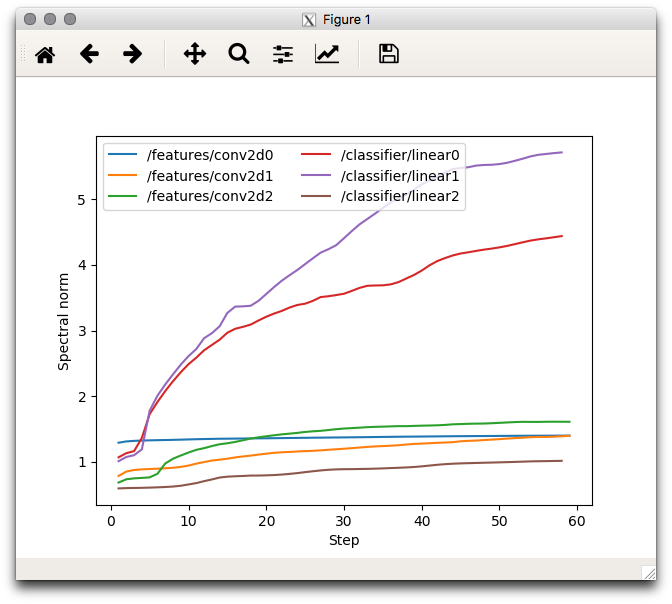
\includegraphics[max width=\textwidth]{gfx/diagrams/software_screens/example_mpl.png}
        \caption{Exemplary view of a Matplotlib figure forwarded over SSH}\label{fig:example_mpl}
    }
\end{subfigure}

\begin{subfigure}{\textwidth}
    \hypertarget{fig:example_tb}{%
        \centering
        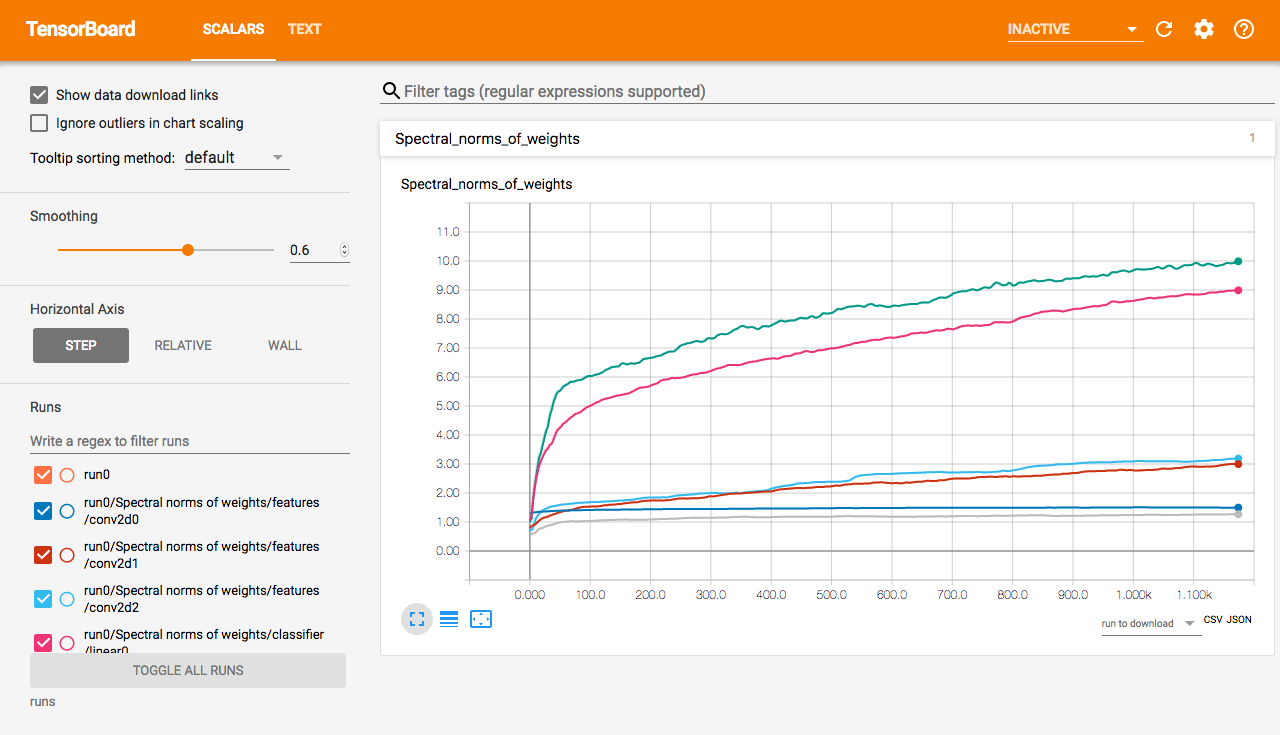
\includegraphics[width=\textwidth]{gfx/diagrams/software_screens/example_tb.png}
        \caption{Exemplary view of a TensorBoard session}\label{fig:example_tb}
    }
\end{subfigure}
\end{figure}

\hypertarget{sec:other-tools}{%
\subsection{Miscellaneous tools}\label{sec:other-tools}}

There are a few modules which simplify development with the library but are not
part of the distribution obtained from PyPi or by running the setup script.

The \texttt{train} package defines a \texttt{Trainer} class which encapsulates
all the logic and parameters needed to train a neural network on one of the
datasets provided with PyTorch. The class's capabilities include the following

\begin{itemize}
    \item
        Look up model and dataset by name
    \item
        Bundle all hyperparameters
    \item
        hook the \texttt{Exporter} into the model for
        publishing data
    \item
        configure the optimisation algorithm to use for training
    \item
        train the model for one batch
\end{itemize}

The \texttt{Trainer} class is used in the main script (\texttt{main.py}), which
serves as a command line interface to the library while developing. When trying
out the library, it can also be used as an initial starting point.

\begin{table}
    \caption{Named arguments to \texttt{main.py}}
    \begin{tabularx}{\linewidth}{lX}
        \toprule
        Parameter                                   & Explanation\tabularnewline
        \midrule
        \lstinline{-m}, \lstinline{--model}         & Model class to train\tabularnewline
        \lstinline{-d}, \lstinline{--dataset}       & Dataset to train on. Possible choices: \lstinline{MNIST}, \lstinline{FashionMNIST}, \lstinline{CIFAR10}, \lstinline{CIFAR100}\tabularnewline
        \lstinline{-b}, \lstinline{--batch-size}    & Default: 128\tabularnewline
        \lstinline{-e}, \lstinline{--epochs}        & Default: 10\tabularnewline
        \lstinline{-o}, \lstinline{--optimizer}     & Optimizer to use. Default: \lstinline{Adam}\tabularnewline
        \lstinline{-a}, \lstinline{--ratio-average} & Number of ratios to average for stability (currently unused). Default: 10\tabularnewline
        \lstinline{-s}, \lstinline{--subsample}     & Number of batches to ignore between updates. Default: \lstinline{1}\tabularnewline
        \lstinline{-v}, \lstinline{--visualisation} & Visualisation backend to use. Possible choices: \lstinline{tb}, \lstinline{mpl}. Default: \lstinline{tb}\tabularnewline
        \lstinline{-V}, \lstinline{--verbose}       & Print training progress. Default: \lstinline{False}\tabularnewline
        \lstinline{--spectral-norm}                 & Use spectral norm subscriber on weights. Default: \lstinline{False}\tabularnewline
        \lstinline{--histogram}                     & Use histogram subscriber(s)\tabularnewline
        \lstinline{--ratio}                         & Use ratio subscriber(s)\tabularnewline
        \lstinline{--test-accuracy}                 & Use test set accuracy subscriber. Default: \lstinline{False}\tabularnewline
        \lstinline{--train-accuracy}                & Use train accuracy subscriber. Default: \lstinline{False}\tabularnewline
        \lstinline{--depth}                         & Depth to which to add modules.  Default: \lstinline{-1}\tabularnewline
        \bottomrule
    \end{tabularx}
\end{table}

The library can be installed to the local Python environment by use of the
provided setuptools script (\texttt{setup.py}). It can also be downloaded from
the \href{https://pypi.org/}{Python Package Index} by use of the package manager
\texttt{pip}:
\begin{lstlisting}[language=Python]
pip install ikkuna
\end{lstlisting}

\hypertarget{plugin-infrastructure}{%
\subsection{Plugin Infrastructure}\label{plugin-infrastructure}}

Among the main selling points of this library is the provision to add new
metrics as plugins and reuse them system-wide for all architectures. Plugins in
Python projects can be enabled through appropriate use of the
\texttt{setuptools} library. During the setup process for installing the
library, entry points (which are names) are defined by the library which can be
used by plugins to announce themselves. \verb+Ikkuna+ provides the
\lstinline[language=Python,breaklines=false]{'ikkuna.export.subscriber'} entry
point. For registering a plugin, the author must simply use that entry point to
make a plugin available. For illustration, \cref{lst:plugin} shows how to setup
a \texttt{setup.py} setuptools file. The plugin can be installed like any other
Python package with \begin{lstlisting}[language=Python] python setup.py install
\end{lstlisting} which will install all required dependencies inside the current
environment. The PyTorch library must be installed manually since the binary
distribution is too old at the time of writing. Detailed instructions can be
found in the user guide which is part of the documentation.

\begin{lstlisting}[label=lst:plugin, language=Python, caption=Sample setup script for subscriber plugins]
#!/usr/bin/env python

from distutils.core import setup
import setuptools

setup(name='<your package name>',
    version='<version>',
    description='<description>',
    author='<your name',
    author_email='<your email>',
    packages=['<package name>'],
    # ... any other args
    entry_points={
        'ikkuna.export.subscriber': [
            'YourSubscriber = module.file:YourSubscriber',
        ]
    })
\end{lstlisting}

\subsection{Documentation}\label{doc}

The entire codebase is liberally documented using the Sphinx documentation
processor\footnote{\url{http://www.sphinx-doc.org/}}. The documentation contains
further documents with a detailed user guide and installation instructions. Sphinx
allows generating documentation in many formats from the same source, most
usefully HTML and PDF. At the time of writing, the HTML documentation and API
reference is hosted at \url{https://peltarion.github.io/ai_ikkuna/}.

\section{Business Case for the Library}\label{business-case}

This work is done in cooperation with Peltarion
AB\footnote{\url{http://www.peltarion.com/}}, a software company based in
Stockholm, Sweden. Peltarion's stated mission is to

\begin{quote}
    [provide] an
    operational AI platform for producing real-world AI applications at scale and at
    speed.
\end{quote}

The Peltarion platform is a web-based deep learning platform with which users
can upload, preprocess and modify datasets, create deep neural architectures
without having to write code and track performance of each model and dataset
version through experiment versioning. Trained models can be directly deployed
as a web service.

The modeling interface presented to the user is shown in \cref{fig:platform}

\begin{figure}
    \centering
    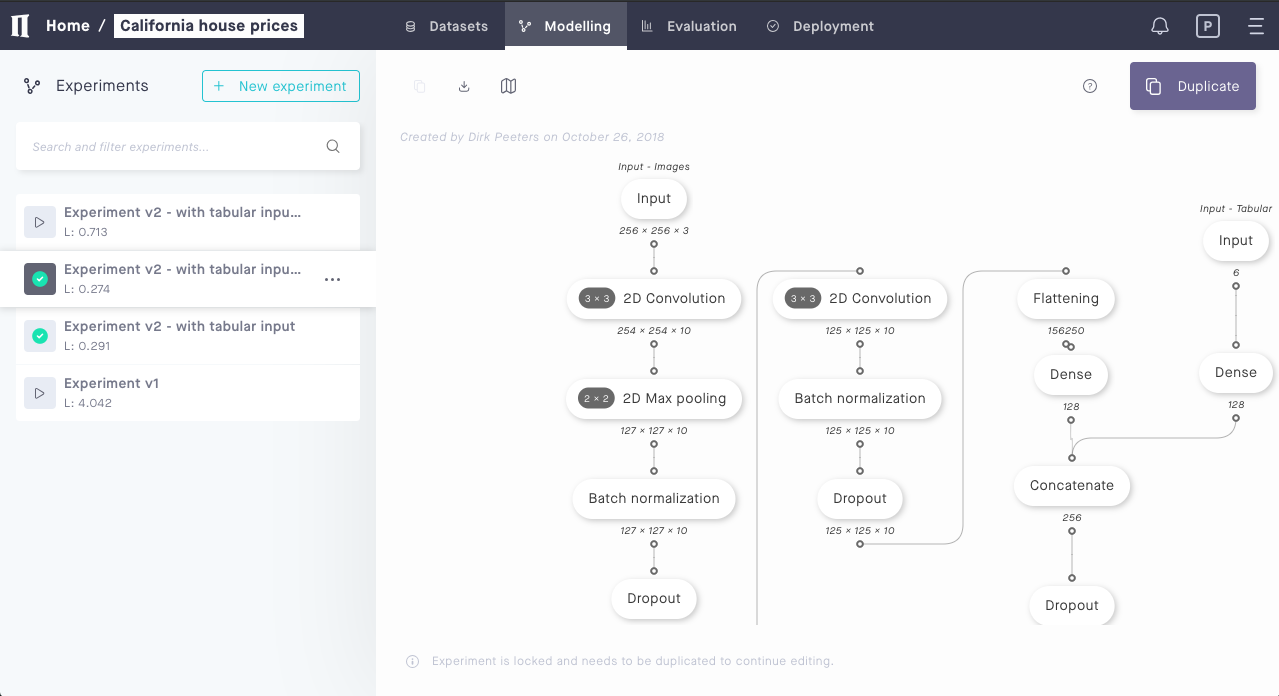
\includegraphics[width=\textwidth]{gfx/diagrams/software_screens/peltarion_platform.png}
    \caption{The Peltarion platform modeling screen}
    \label{fig:platform}
\end{figure}

While the product in question is code-free for the user, it is powered by a deep
learning framework on the server side. The business proposition made by
Peltarion is to make training deep neural networks more affordable, which the
company wants to realise through savings in development time from problem
statement to model deployment. As outlined in \cref{sec:motivation}, development
of state-of-the art deep learning applications requires both expertise and
education as well as experience. Since experts in any discipline are rare and
expensive, lowering the cost in this area requires simplifying the process of
creating deep learning solutions. A code-free platform is one way to accomplish
this and make deep learning more accessible to users and companies without the
previously required expertise in research and engineering.

This thesis ties into this objective in two ways. Firstly, by providing an API against
which training metrics can easily be implemented and served to arbitrary
backends, engineering effort for metric features of the platform could be reduced. For
this work, plotting backends have been implemented, but the decoupled compontent
architecture of the \texttt{ikkuna} library was chosen precisely to enable
arbitrary data sinks for the computed metrics, for instance a web service or a
database which is accessed by the Peltarion platform to display metrics to the
user. The engineering team at Peltarion could make use of this library to handle
metric logging on arbitrary models created by the platform's users without
having to resort to code generation during translation of the abstract model
definition created in the browser to the model implementation in the backend.

Secondly, the library -- or the ideas prototyped therein -- will be helpful in
providing feedback to the user about the state of their experiment. Since the
platform is at least partially aimed at non-experts, even well-known and simple
metrics can be of great help in avoiding common pitfalls in model training. This
directly reduces the opaqueness of the training process to the non-expert user,
reducing time wasted on fruitless experiments and increasing confidences in the
product.

It should be stressed, however, that the software implemented for this thesis is
free and open-source and not owned or licensed by Peltarion AB.
